\chapter{Spanning Trees and How to find them}
Rishnak found Ajur and Jura walking along a stretch of road with trees on either side of the road. Rishnak remembered about his interaction with him about trees. But there is one kind of tree in a graph that Rishnak wanted to Ajur today.
In a connected graph $G=(V,E)$ (connected means that there is a path between every pairs of vertices in $G$), a tree (spanning all the vertices) is a subgraph =$T(V,E_1)$ of G satisfying the two conditions
\begin{enumerate}
    \item The subgraph, T,  is a tree (i.e., contains no cycles and of course connected; i.e., there is only one path between every pair of vertices.
    \item Vertex set of $T$ is the same as the vertex set of $G$.
\end{enumerate}

Here is an example of Graph Figure \ref{11g1} and a subgraph of this graph which is a spanning tree shown in Figure \ref{11g2} 
\begin{figure}
\begin{center}
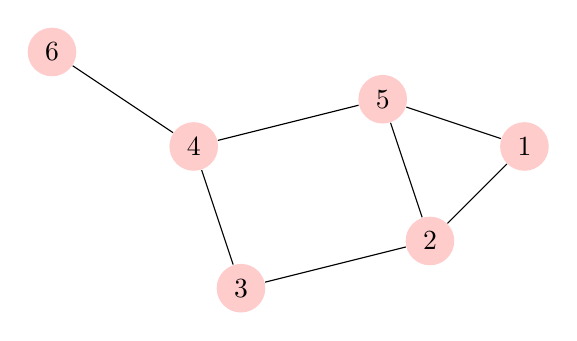
\begin{tikzpicture}
  [scale=.6,auto=left,every node/.style={circle,fill=red!20}]
  \node (n6) at (1,10) {6};
  \node (n4) at (4,8)  {4};
  \node (n5) at (8,9)  {5};
  \node (n1) at (11,8) {1};
  \node (n2) at (9,6)  {2};
  \node (n3) at (5,5)  {3};

  \foreach \from/\to in {n6/n4,n4/n5,n5/n1,n1/n2,n2/n5,n2/n3,n3/n4}
    \draw (\from) -- (\to);

\end{tikzpicture}
\caption{ Example Graph with 6 vertices and 7 edges}\label{11g1}
\end{center}
\end{figure}
\begin{figure}
\begin{center}
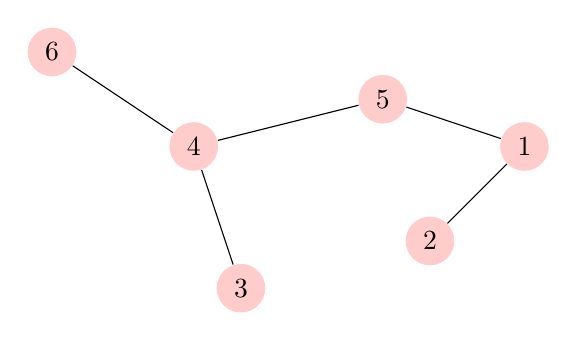
\begin{tikzpicture}
  [scale=.6,auto=left,every node/.style={circle,fill=red!20}]
  \node (n6) at (1,10) {6};
  \node (n4) at (4,8)  {4};
  \node (n5) at (8,9)  {5};
  \node (n1) at (11,8) {1};
  \node (n2) at (9,6)  {2};
  \node (n3) at (5,5)  {3};

  \foreach \from/\to in {n6/n4,n4/n5,n5/n1,n1/n2,n3/n4}
    \draw (\from) -- (\to);

\end{tikzpicture}
\caption{ Subgraph of \ref{11g1} which is a spanning tree of \ref{11g1} - Spanning tree has 6 vertices and 5 edges}\label{11g2}
\end{center}
\end{figure}
Rishnak asked Ajur whether he can construct one more spanning tree for this greaph \ref{11g1}. Ajur was eager to show off and drew the following graph \ref{11g3}
\begin{figure}
\begin{center}
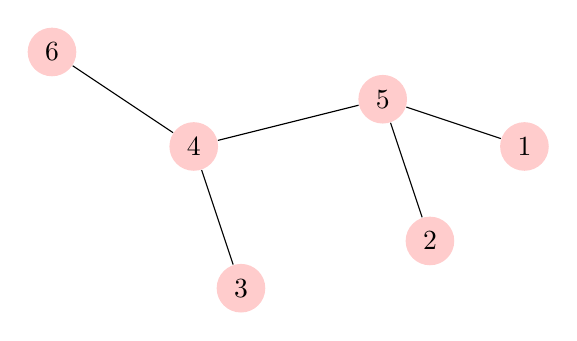
\begin{tikzpicture}
  [scale=.6,auto=left,every node/.style={circle,fill=red!20}]
  \node (n6) at (1,10) {6};
  \node (n4) at (4,8)  {4};
  \node (n5) at (8,9)  {5};
  \node (n1) at (11,8) {1};
  \node (n2) at (9,6)  {2};
  \node (n3) at (5,5)  {3};

  \foreach \from/\to in {n6/n4,n4/n5,n5/n1,n2/n5,n3/n4}
    \draw (\from) -- (\to);

\end{tikzpicture}
\caption{ Another Spanning Tree of Graph in \ref{11g1}}\label{11g3}
\end{center}
\end{figure}

Rishnak asked Ajur how many distinct spanning trees (labelled non isomorphic) are there with a sneer. Ajur had an answer for this too. There are two cycles in this graph, namely (2,3,4,5) and (1,5,2). One is of 
length 4 and the other is of length 3. But they share a common edge (2,5). There are 4 possible spanning trees with a cycle of length 4 and there are 2 possibilities to choose from the other cycle - giving rise to 8 spanning trees. They are enumerated.   
The edge (4,6) has to be present in every spanning tree. The eight spanning tree edges are given below.
\begin{enumerate}
    \item \{(4,6),(4,5),(5,2),(2,3),(5,1)\}
    \item \{(4,6),(4,5),(5,2),(2,3),(2,1)\}
    \item \{(4,6),(4,5),(4,3),(5,2),(5,1)\}
    \item \{(4,6),(4,5),(4,3),(5,2),(2,1)\}
    \item \{(4,6),(4,5),(2,3),(5,2),(5,1)\}
    \item \{(4,6),(4,5),(4,3),(5,2),(2,1)\}
    \item \{(4,6),(4,5),(4,3),(2,3),(5,1)\}
    \item \{(4,6),(4,5),(4,3),(2,3),(2,1)\}
\end{enumerate}

Ajur asked what is the maximum number of labeled spanning trees in a graph with $n$ vertices. Ajur further added that the maximum number of spanning trees will be present in a complete graph as there have the maximum number of edges in a $n$ vertex graph. Rishnak agreed that the complete trees have the largest number of spanning trees. We can find the number of spanning trees in a complete graph using Pr{\"u}fer code (which we talked about a couple of days ago) in Chapter 8. Ajur remembered that and interjected for a $n$ vertex tree, you need only a Pr{\"u}fer code of length $n-2$. Rishnak said that is correct that the Pr{\"u}fer code is of length $n-2$ for a $n$ vertex graph. Each of the $n-2$ characters in a code to be any of the $n$ vertices. Hence the number of (labeled) spanning trees in a complete graph with $n$ vertices is $n^{n-2}$.

Since there are $n-1$ edges in a spanning tree, each of the remaining $e-n+1$ edges when taken with a spanning tree will create a cycle. Thus there will be $s-n+1$ cycles. These cycles are called Fundamental cycles. Each fundamental cycle has exactly one non spanning tree edge. \footnote{Euler's equation \ref{eqn:euler} in chapter 9 uses this fact}. Rishnak showed with an example Figure \ref{11g4}.

\begin{figure}
\begin{center}
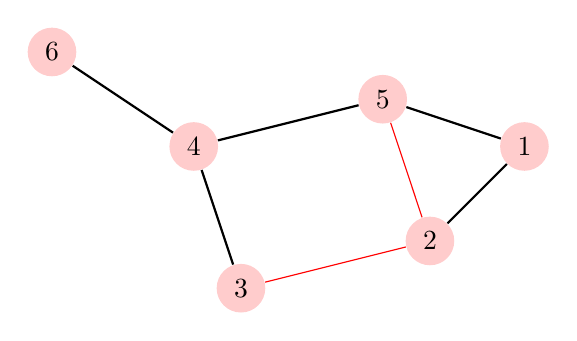
\begin{tikzpicture}
  [scale=.6,auto=left,every node/.style={circle,fill=red!20}]
  \node (n6) at (1,10) {6};
  \node (n4) at (4,8)  {4};
  \node (n5) at (8,9)  {5};
  \node (n1) at (11,8) {1};
  \node (n2) at (9,6)  {2};
  \node (n3) at (5,5)  {3};

  \foreach \from/\to in {n6/n4,n4/n5,n5/n1,n1/n2,n3/n4}
    \draw [thick] (\from) -- (\to);
  \foreach \from/\to in {n5/n2,n2/n3}
   \draw [color=red] (\from) -- (\to);
\end{tikzpicture}
\caption{ Two fundamental cycles of \ref{11g1} with respect to a spanning tree of \ref{11g2} - Spanning tree edges are shown as thick lines and nonspanning tree edges are shown in red color. Fundamental Cycles are (1,2,5) and (4,5,1,2,3)}\label{11g4}
\end{center}
\end{figure}